\section{EXPERIMENTS}
\label{experiments}

\subsection{Toy examples}

We consider three differents LVGGM with $p=45$ observed variables, with a tree structure on observed variables and the following structure on latent variables :
\begin{itemize}
\item \textit{model 1}: consists of $h=3$ latent variables, we split observed variables in three groups of size $15$ and connect each group to a single latent variable.
\item \textit{model 2}: consists of $h=3$ latents variables we split observed variables in three groups of different sizes ($20,15$ and $10$) and connect each group to a single latent variable.
\item \textit{model 3}: consists of of $h=4$ latent variables. We select $4$ overlapping groups of size $15$ of observed variables, with a $0.26$ overlap, and connect each one of them to a different latent variable.
\end{itemize}

%- \textit{model 1}: consists of $h=3$ latent variables, we split observed variables in three groups of size $15$ and connect each group to a single latent variable.\\
%- \textit{model 2}: consists of $h=3$ latents variables we split observed variables in three groups of different sizes ($20,15$ and $10$) and connect each group to a single latent variable.\\
%- \textit{model 3}: consists of of $h=4$ latent variables. We select $4$ overlapping groups of size $15$ of observed variables, with a $0.26$ overlap, and connect each one of them to a different latent variable.\\

We generate $50\times p$ samples for each model. Figure \ref{fig:synth} shows the estimated complete concentration matrix obtained for our formulation with the score matching loss compared to a regularization $\ell_1+\tr$, as in \citet{chandrasekaran2010}. For  the $\ell_1+\tr$ regularization we perform an SVD on the obtained low rank matrix to visualize the effect of latent variables. For the first two models the size of the blocks is fixed and for the third model we use the extention of the introduced matrix norm $\Omega_{k,\succeq}$ where the blocks can have different sizes, see section \ref{subsec:norm},  and each size $k$ is penalized by $w_{k}=\sqrt{k}$, see section \ref{subsec:norm}. The regularization parameters are chosen so to recover the desired sparsity pattern for the sparse component and rank for the low rank component.  The decomposition of the low rank component for $\ell_1+\tr$ regularization is not unique so this method cannot recover the effect of latent variables. Both methods recover the sparsity pattern of $S$ and only our methods recovers the structure of the effects of latent variables.

%\begin{figure}[h]
%  \begin{minipage}[ccc]{\linewidth}
%  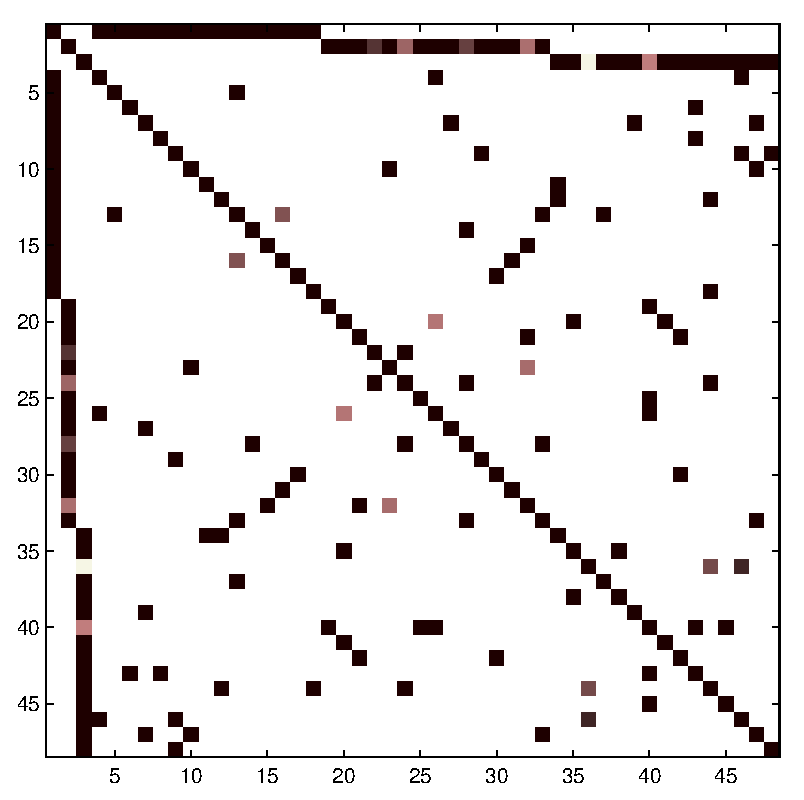
\includegraphics[width=3cm]{fig/disjoint_om}
%  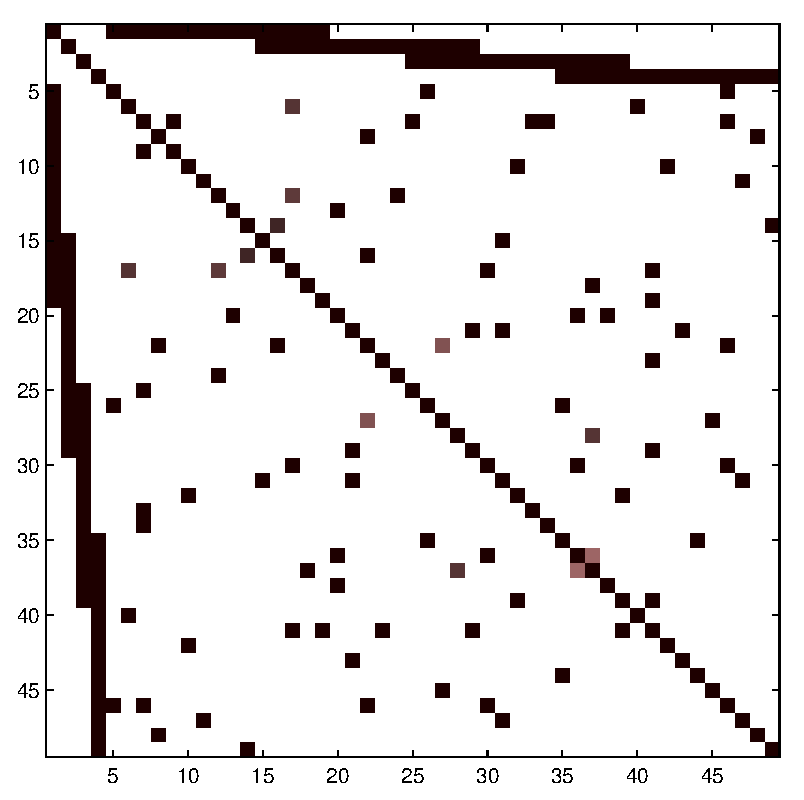
\includegraphics[width=3cm]{fig/overlap_om}
%  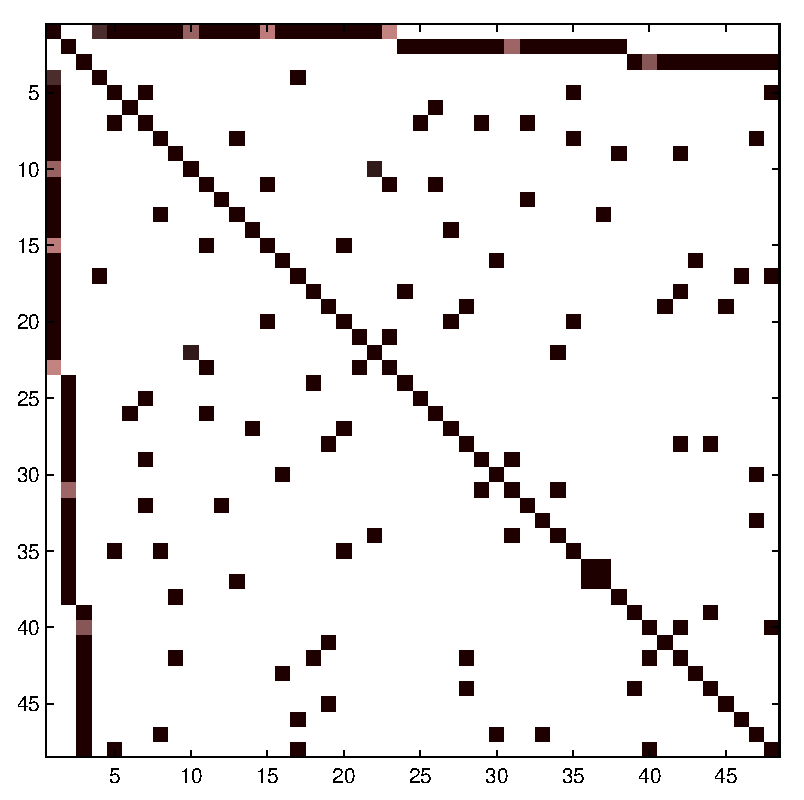
\includegraphics[width=3cm]{fig/diff_om}
%  \end{minipage}
%  \begin{minipage}[ccc]{\linewidth}
%  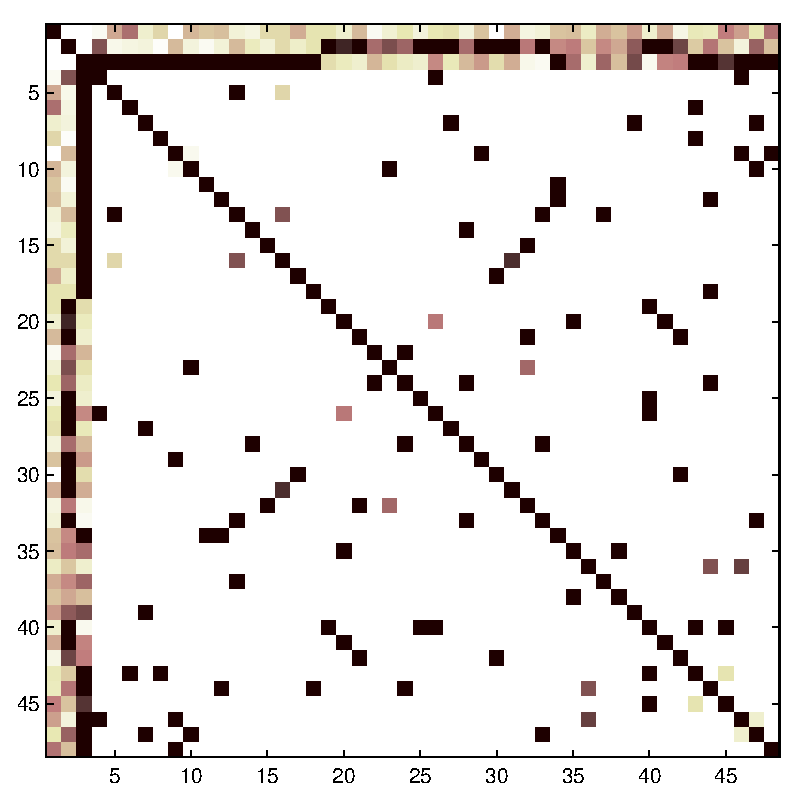
\includegraphics[width=3cm]{fig/disjoint_tr}
%  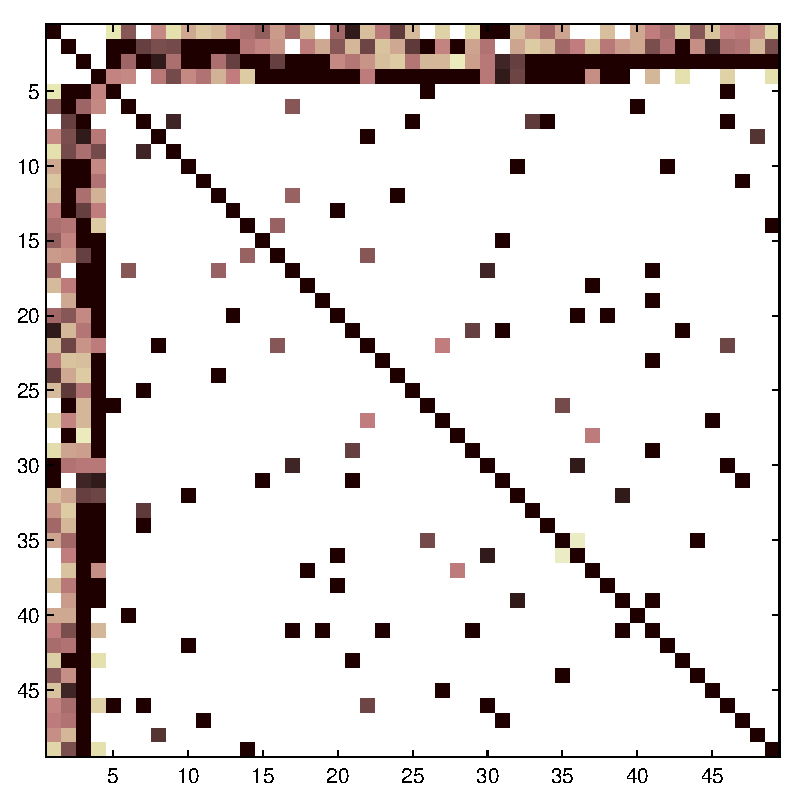
\includegraphics[width=3cm]{fig/overlap_tr}
%  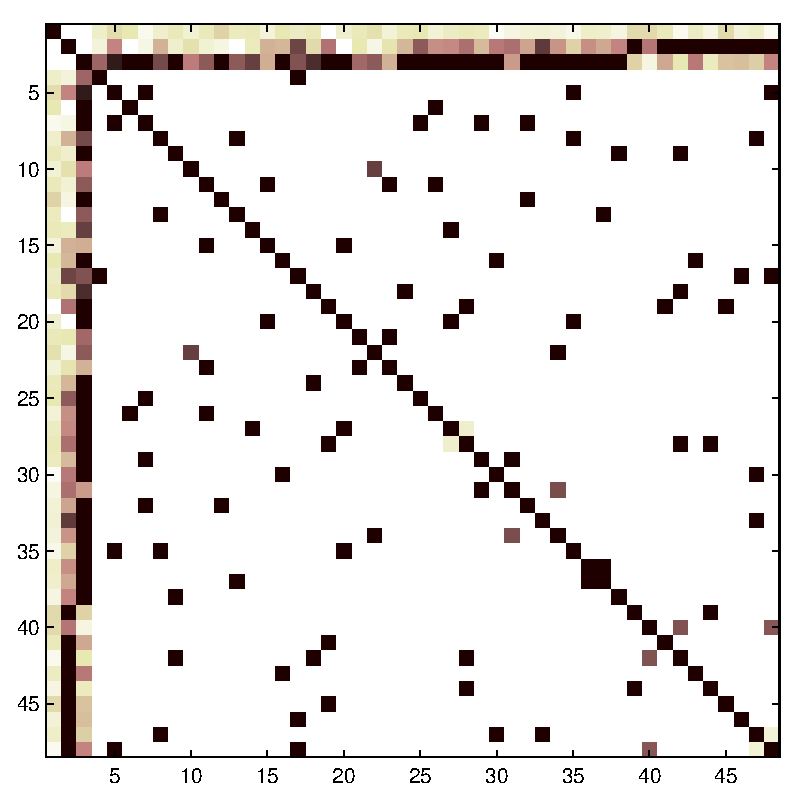
\includegraphics[width=3cm]{fig/diff_tr}
%  \end{minipage}
%  \caption{Experiment for the $k$-chain group Lasso. Top:number of pivots, i.e., drop/full step in active set. Left figure shows the number of pivots per active set call and right plot shows the total number of pivots during iterations. Bottom: evolution of the number of active atoms in our algorithm.}
%\end{figure}

%\begin{figure}
%\center
%\hfill
%\subfigure[Title A]{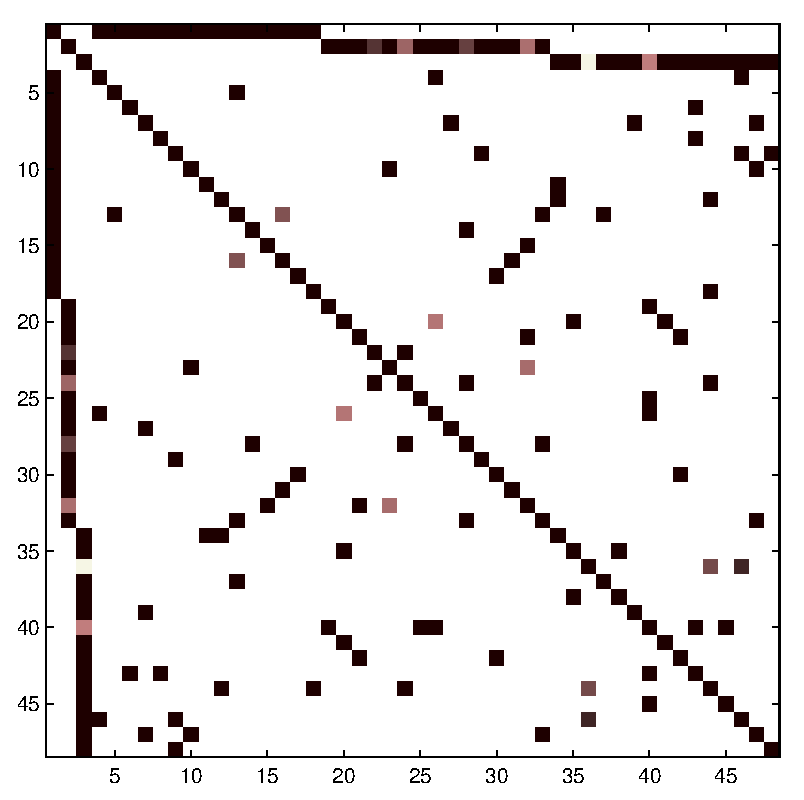
\includegraphics[width=3cm]{fig/disjoint_om}}
%\hfill
%\subfigure[Title B]{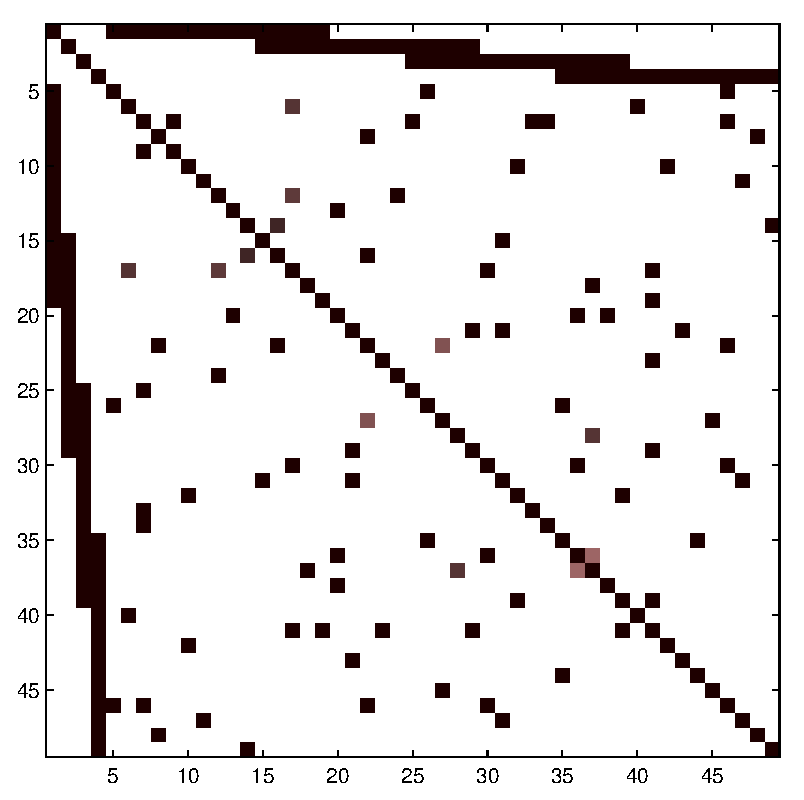
\includegraphics[width=3cm]{fig/overlap_om}}
%\hfill
%\subfigure[Title C]{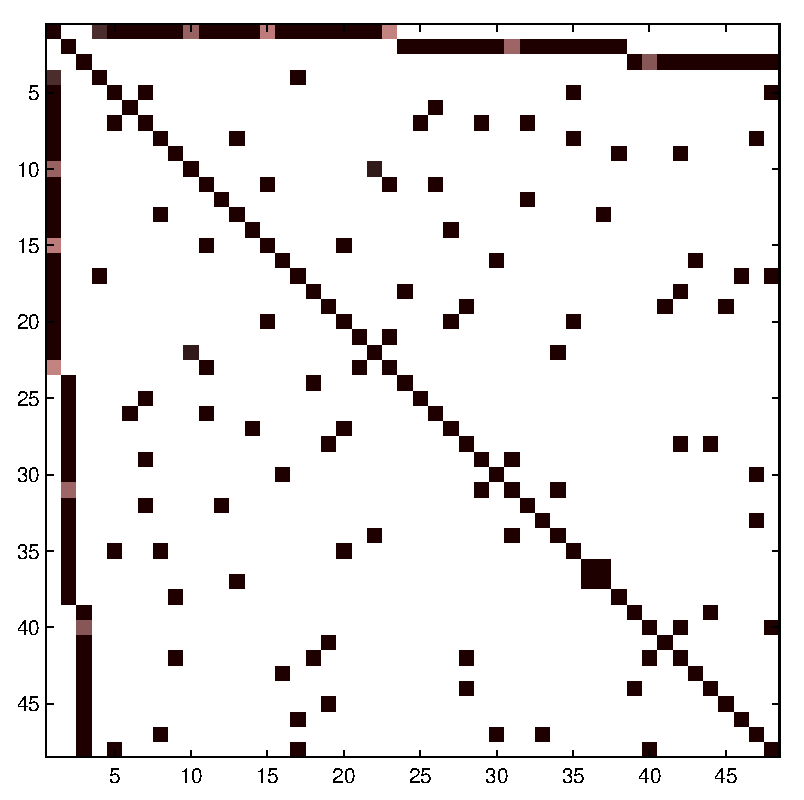
\includegraphics[width=3cm]{fig/diff_om}}
%\hfill
%\\
%\subfigure[Title A]{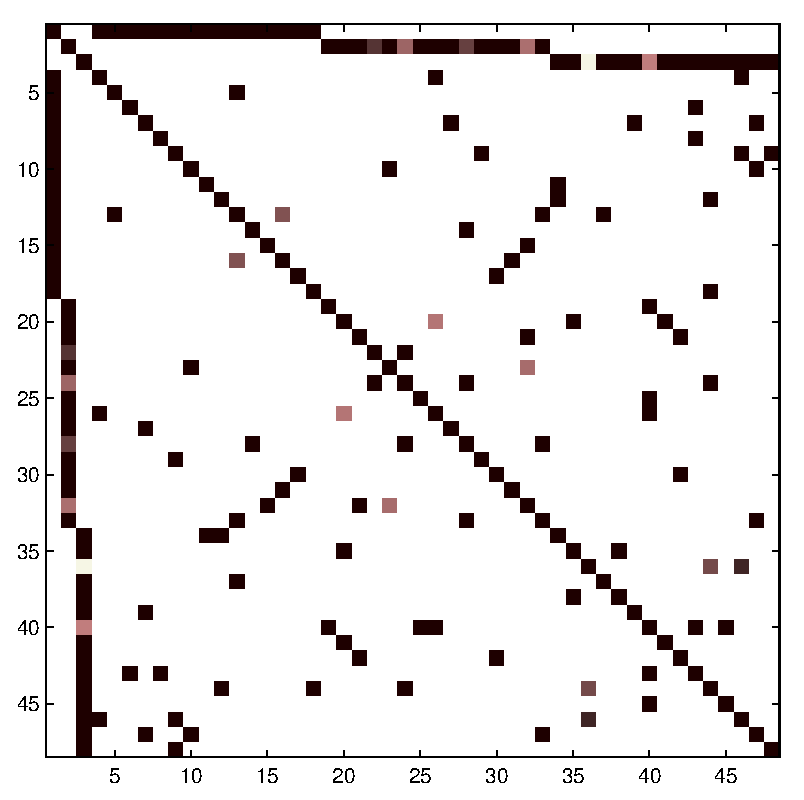
\includegraphics[width=3cm]{fig/disjoint_om}}
%\hfill
%\subfigure[Title B]{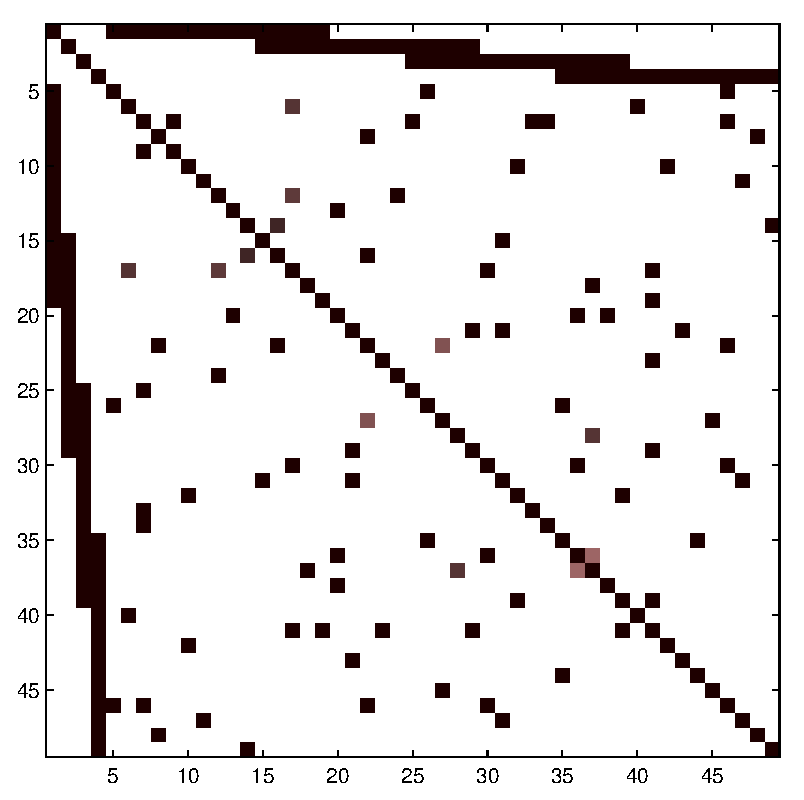
\includegraphics[width=3cm]{fig/overlap_om}}
%\hfill
%\subfigure[Title C]{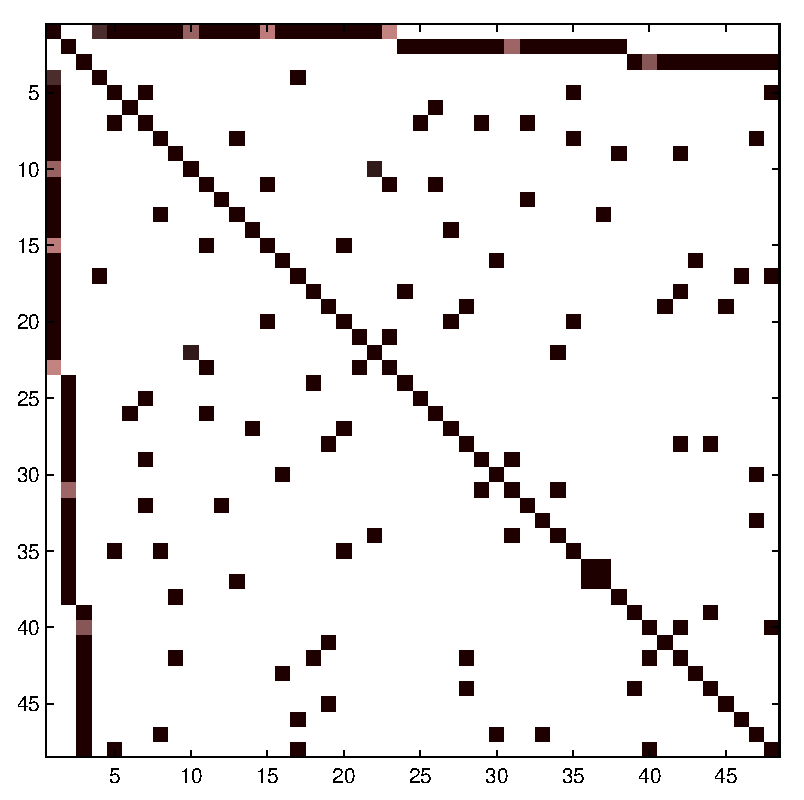
\includegraphics[width=3cm]{fig/diff_om}}
%\hfill
%\caption{Title for both}
%\end{figure}

%\begin{figure}
%\center
%\hfill
%\subfigure[Title A]{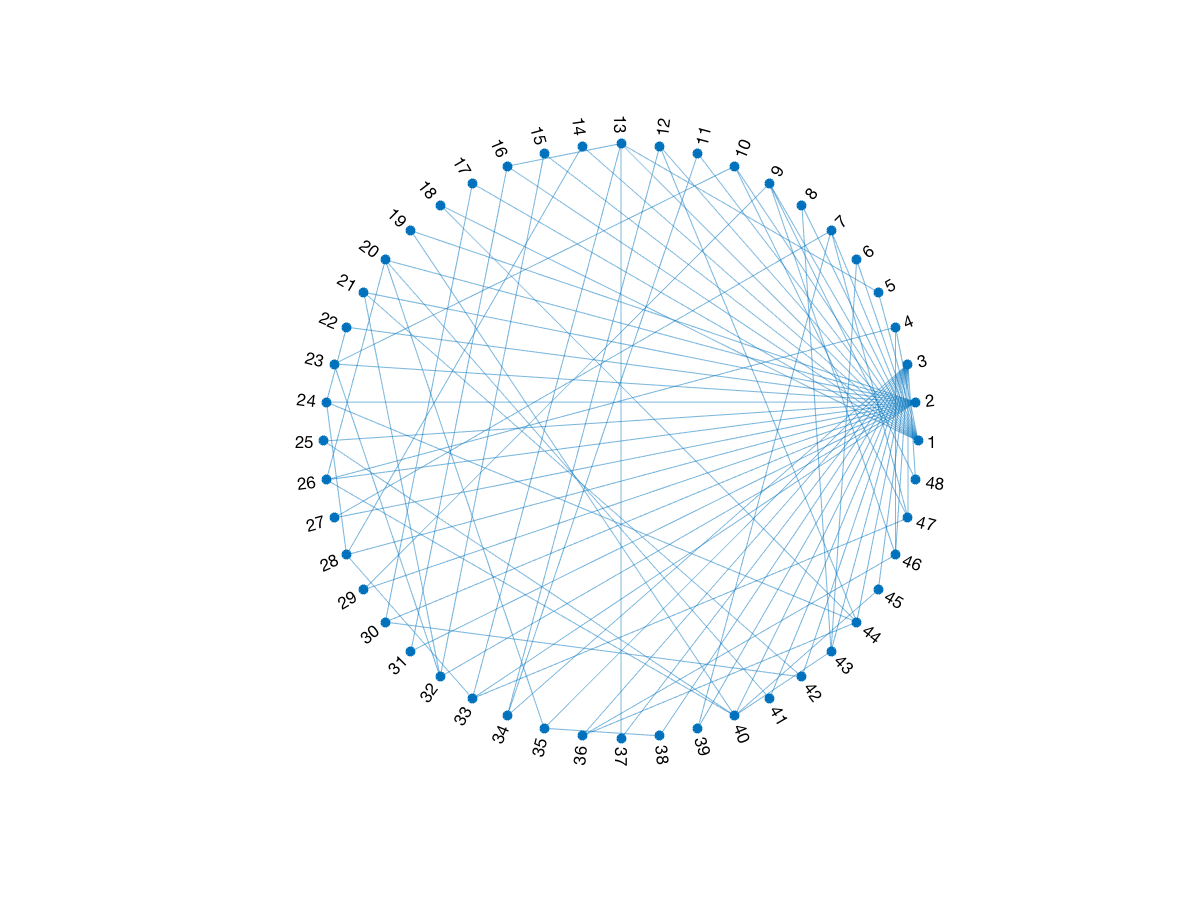
\includegraphics[width=4cm]{fig/disjoint_graph}}
%\hfill
%\subfigure[Title B]{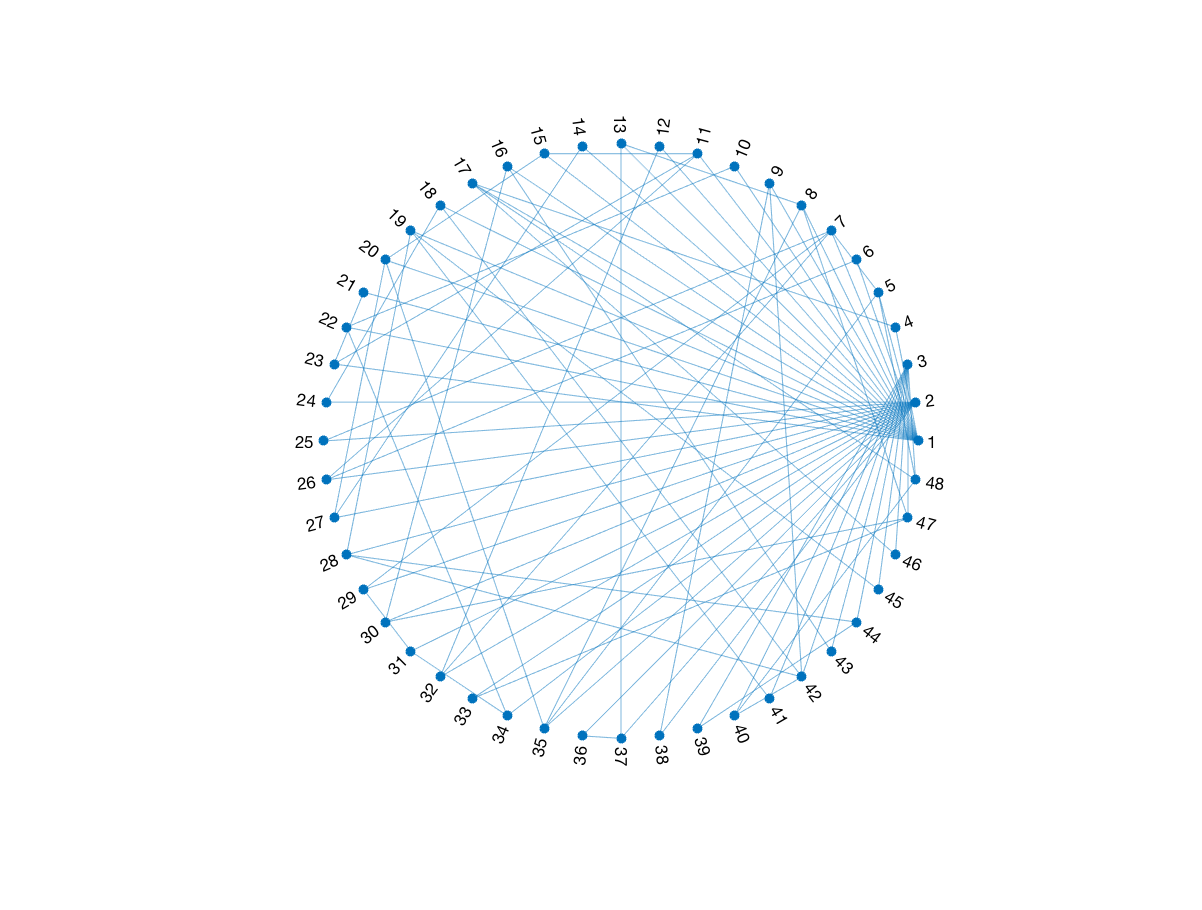
\includegraphics[width=4cm]{fig/diff_graph}}
%\hfill
%\subfigure[Title C]{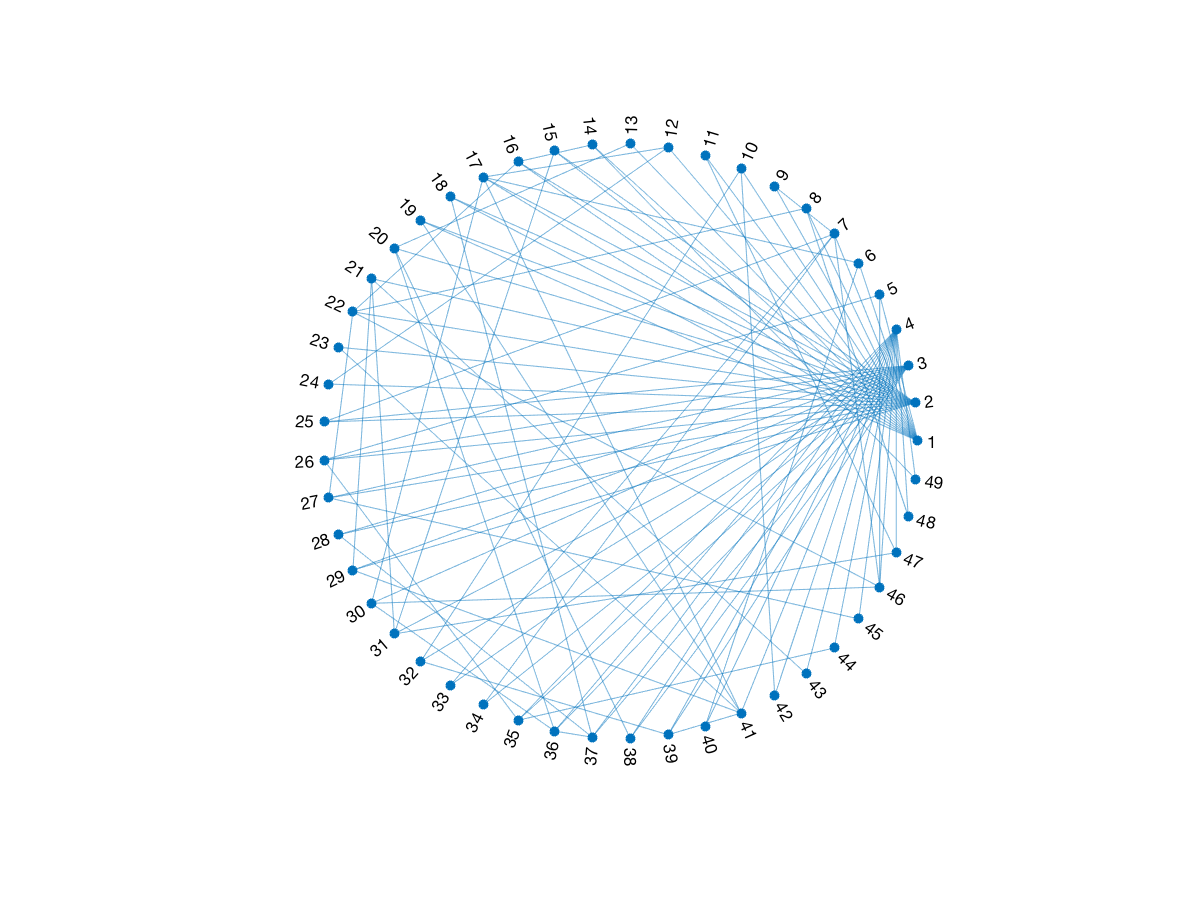
\includegraphics[width=4cm]{fig/over_graph}}
%\caption{Title for both}
%\end{figure}

%\begin{figure}
%\label{fig:synth}
%\center
%\hfill
%\subfigure[ours]{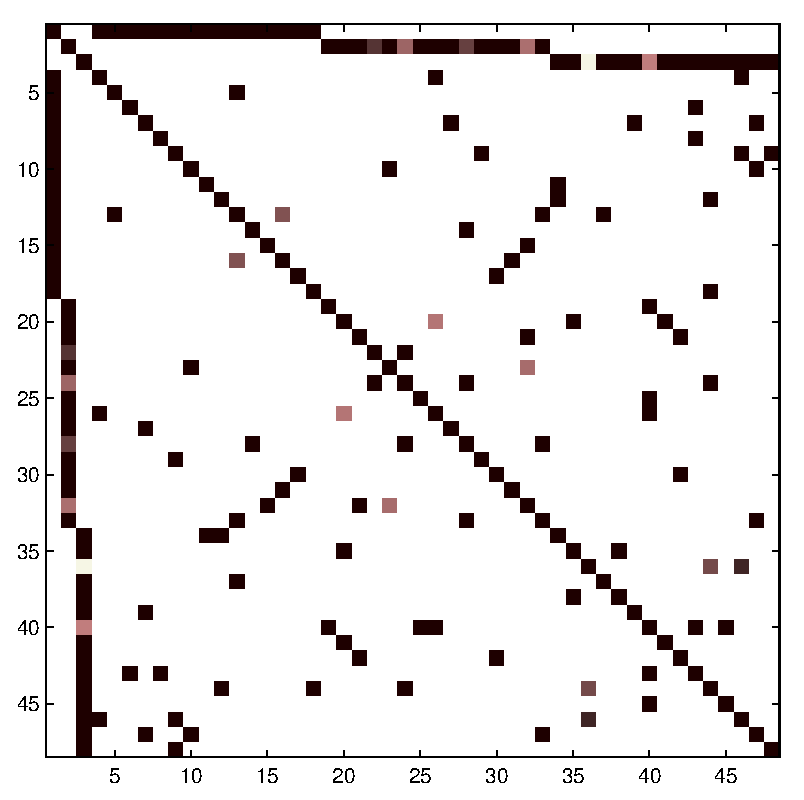
\includegraphics[width=2.2cm]{fig/disjoint_om}}
%\hfill
%\subfigure[$\ell_1+\tr$]{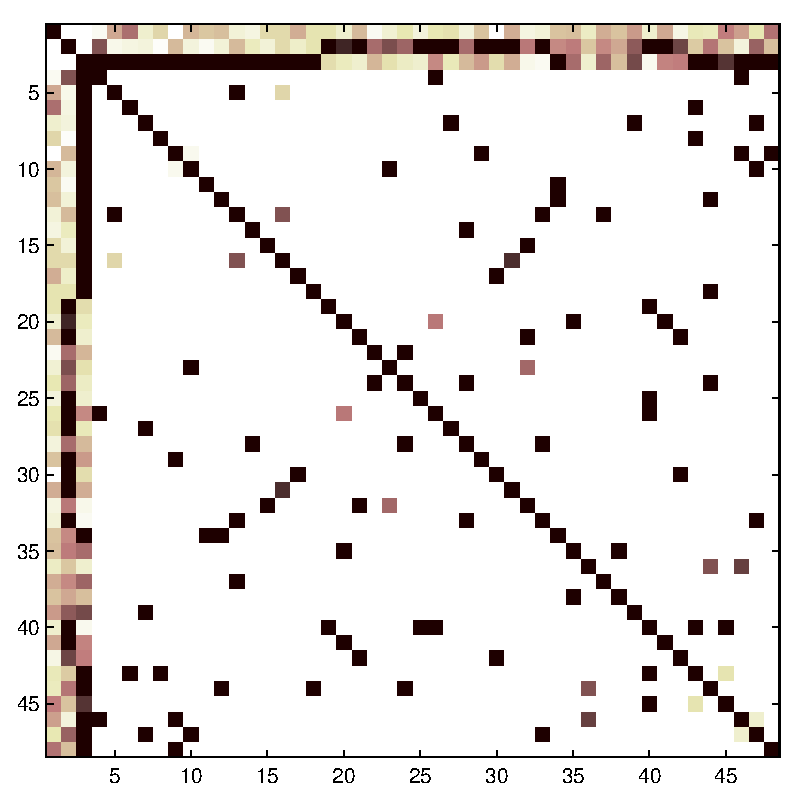
\includegraphics[width=2.2cm]{fig/disjoint_tr}}
%\hfill
%\subfigure[ours]{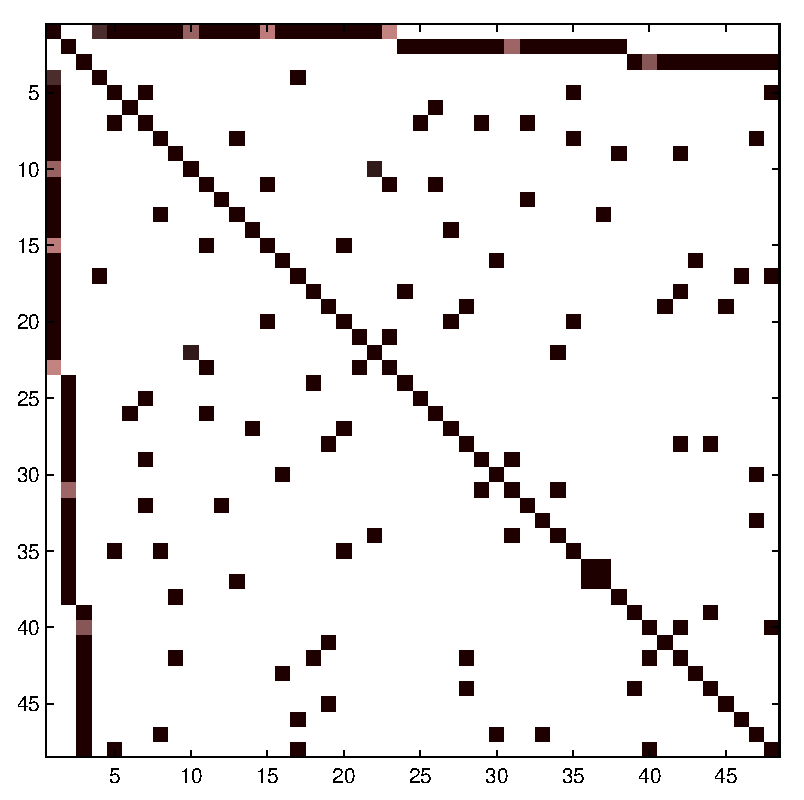
\includegraphics[width=2.2cm]{fig/diff_om}}
%\hfill
%\\
%\subfigure[$\ell_1+\tr$]{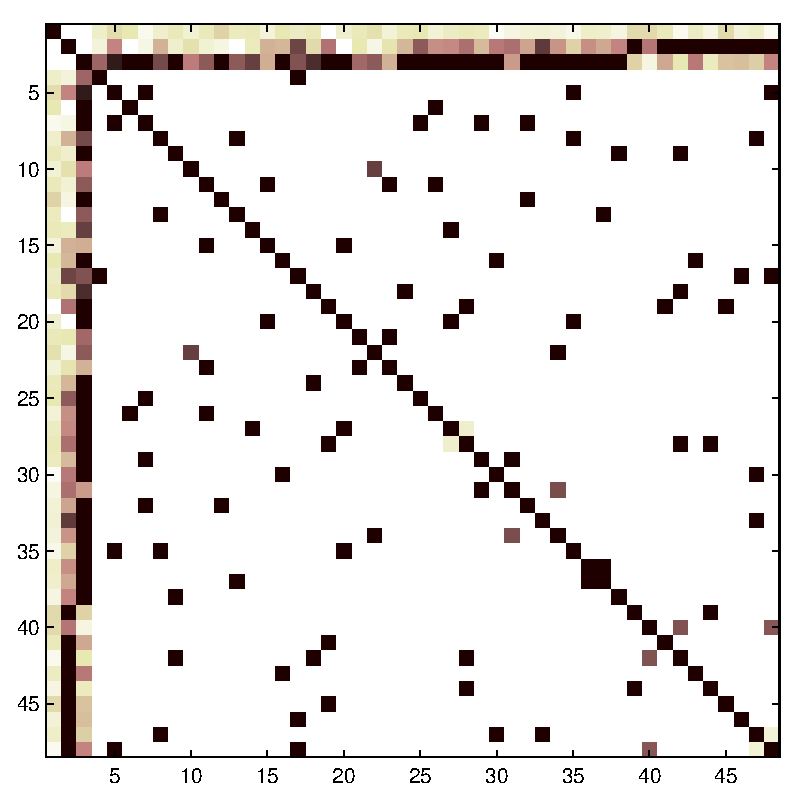
\includegraphics[width=2.2cm]{fig/diff_tr}}
%\hfill
%\subfigure[ours]{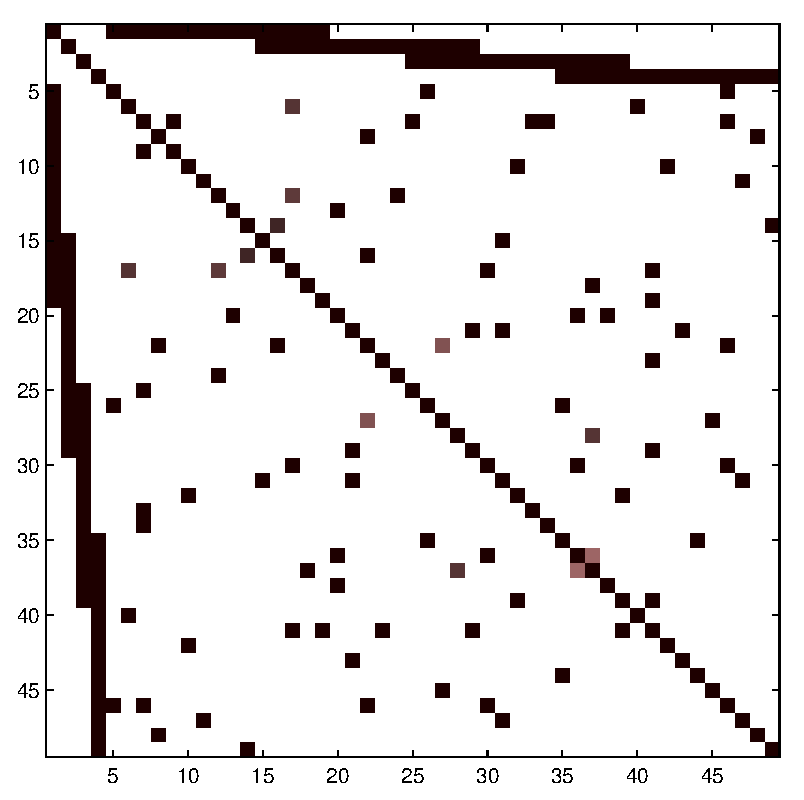
\includegraphics[width=2.2cm]{fig/overlap_om}}
%\hfill
%\subfigure[$\ell_1+\tr$]{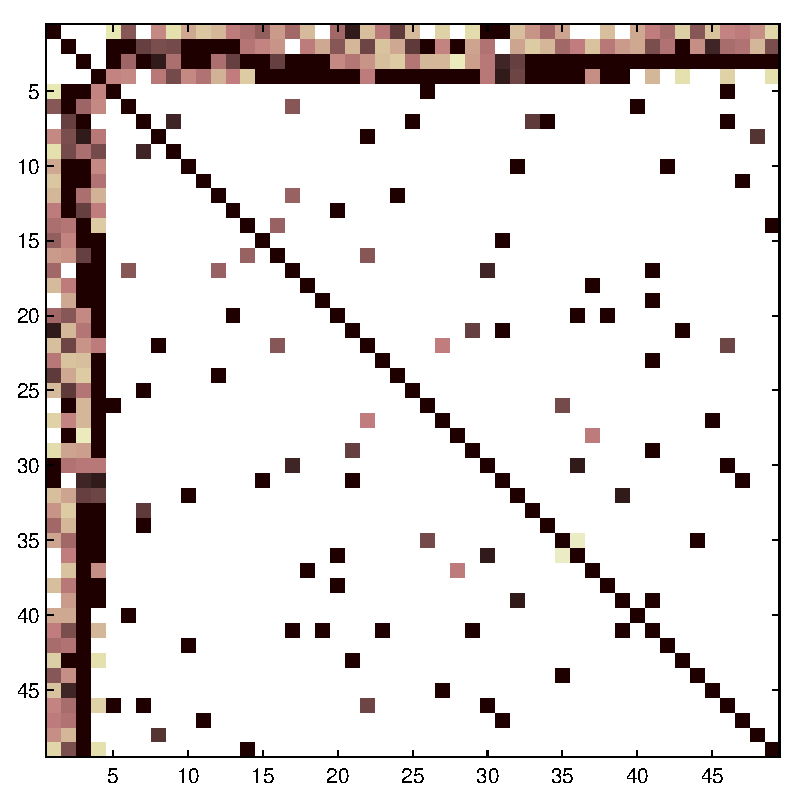
\includegraphics[width=2.2cm]{fig/overlap_tr}}
%\hfill
%\caption{Estimated complete concentration matrices: for \textit{model 1} in (a) ours and (b) $\ell_1+\tr$ regularization; for \textit{model 2} in (c) ours and (d) $\ell_1+\tr$ regularization; for \textit{model 3} in (e) ours and (f) $\ell_1+\tr$ regularization }
%\end{figure}

\begin{figure}
\label{fig:synth}
\center
\begin{tabular}{cc}
    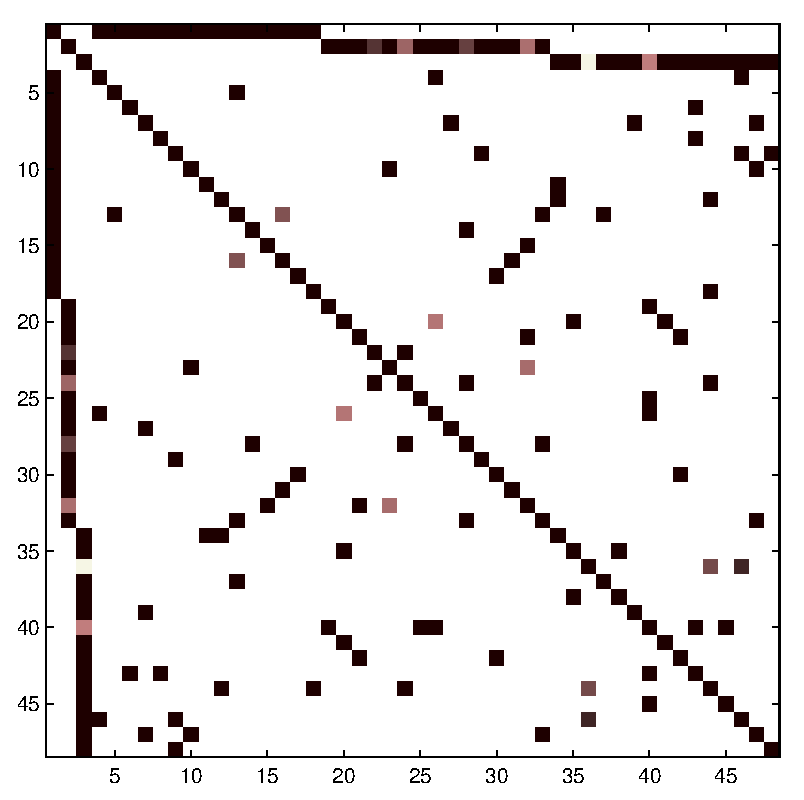
\includegraphics[width=3.5cm]{fig/disjoint_om} 
  & 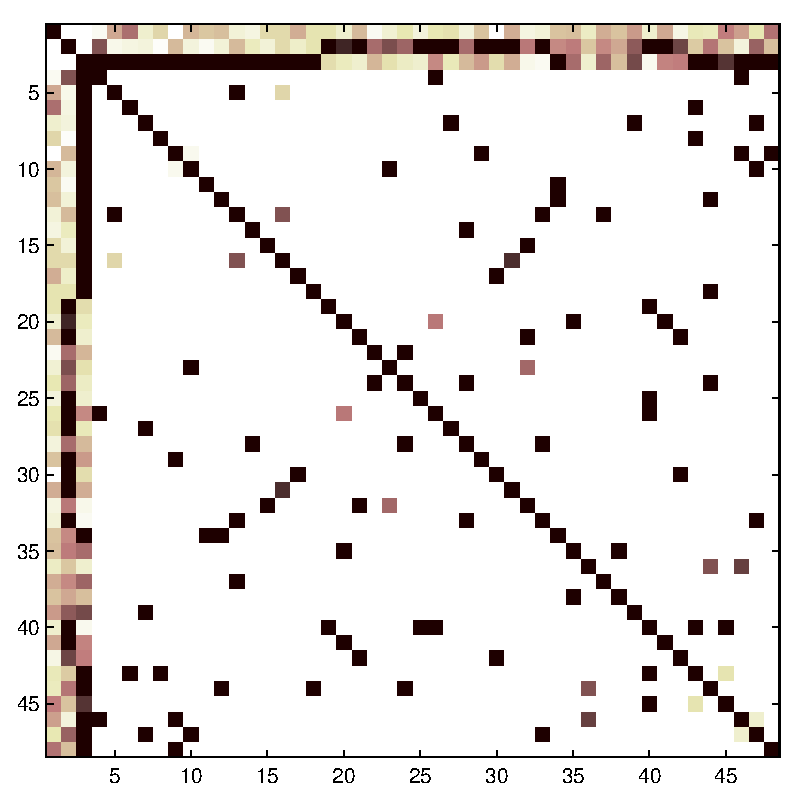
\includegraphics[width=3.5cm]{fig/disjoint_tr} 
   \\    (a) \textit{model 1}, ours & (d)  \textit{model 1}, $\ell_1+\tr$ \\[6pt]
      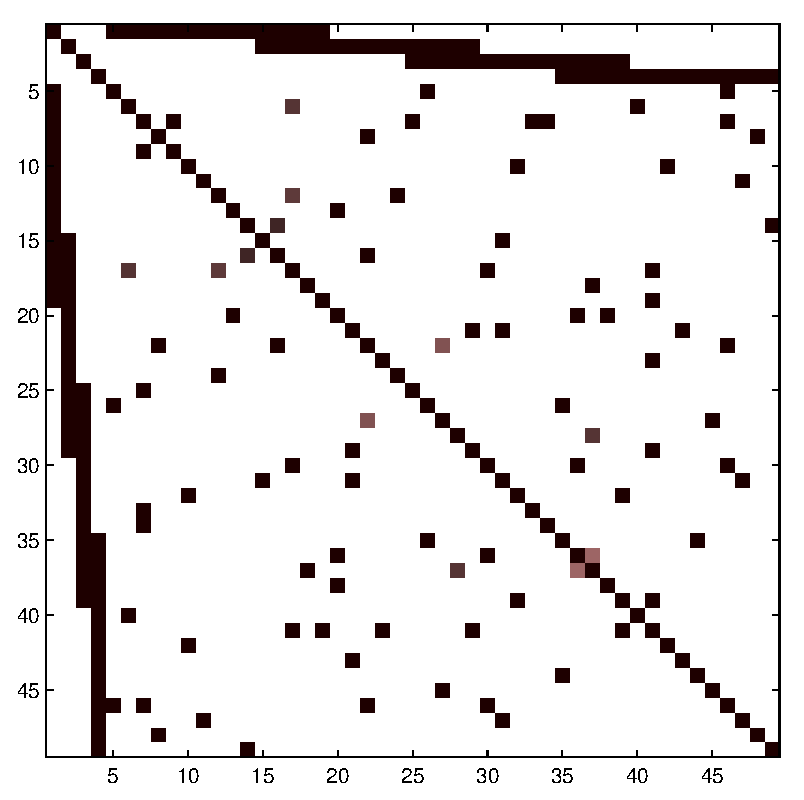
\includegraphics[width=3.5cm]{fig/overlap_om}
  &   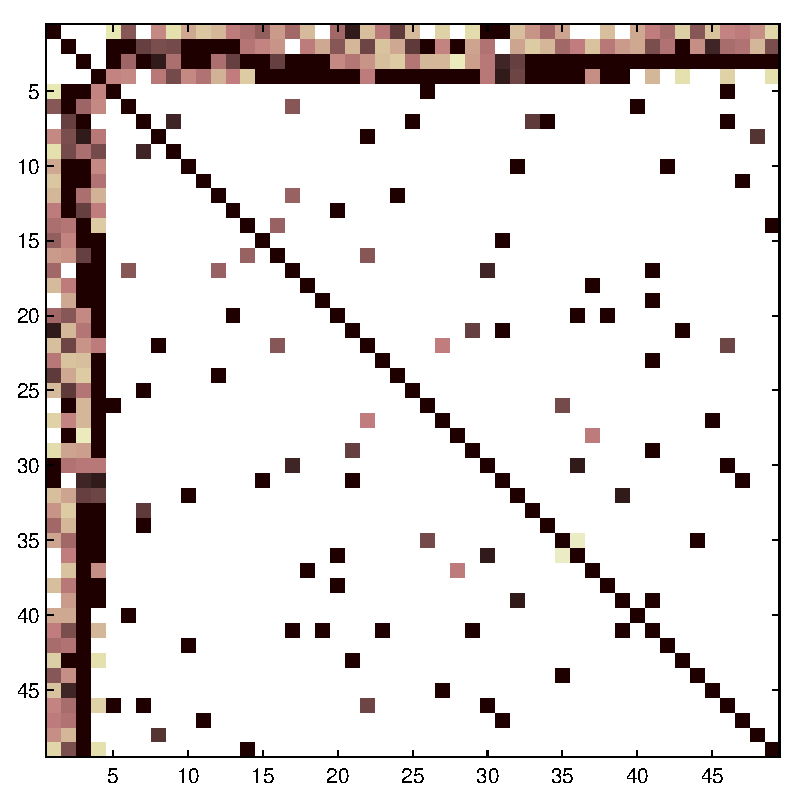
\includegraphics[width=3.5cm]{fig/overlap_tr}
   \\    (b)  \textit{model 2}, ours   & (e)  \textit{model 2}, $\ell_1+\tr$    \\[6pt]
      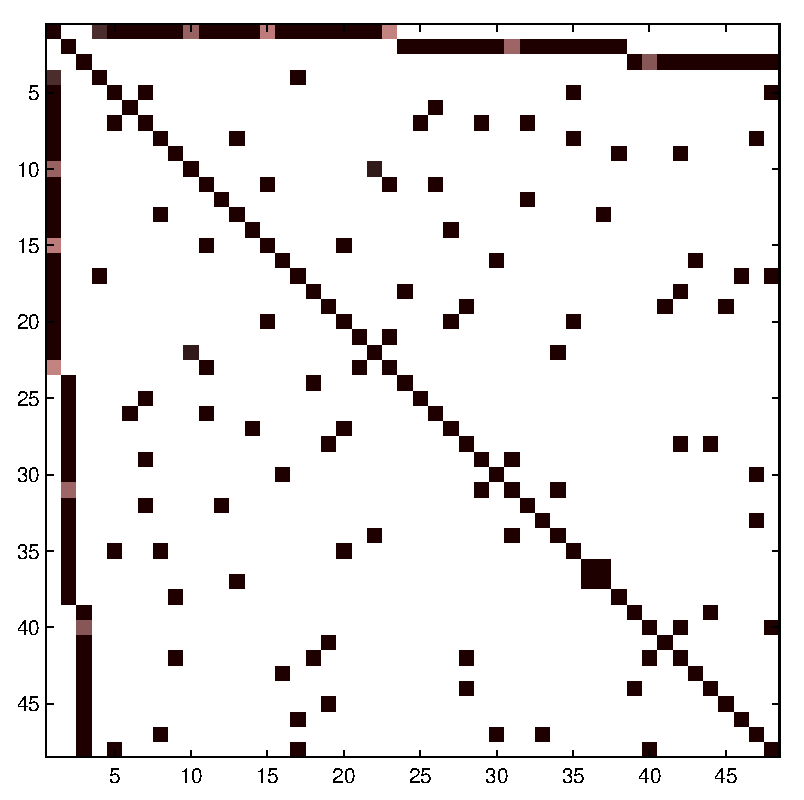
\includegraphics[width=3.5cm]{fig/diff_om}
  &   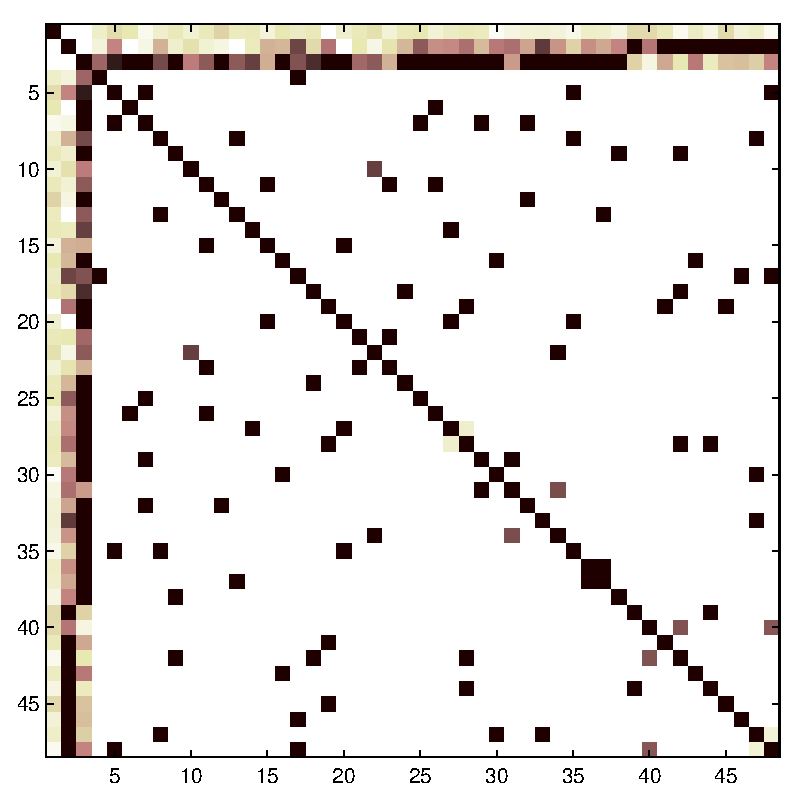
\includegraphics[width=3.5cm]{fig/diff_tr}
   \\    (c)  \textit{model 3}, ours & (f)  \textit{model 3}, $\ell_1+\tr$  \\[6pt]
\end{tabular}
\caption{Estimated $|K_{ij}|$, for $K$ the complete concentration matrices where the three (resp. four) first rows and columns correspond to the latent variables of \textit{model 1} and \textit{model 3} (resp. \textit{model 2}) : for \textit{model 1} in (a) ours and (d) $\ell_1+\tr$ regularization; for \textit{model 2} in (b) ours and (e) $\ell_1+\tr$ regularization; for \textit{model 3} in (c) ours and (f) $\ell_1+\tr$ regularization }
\end{figure}

\section{Synthetic experiments \TODO{on large models}}

\paragraph{Sparse Wishart matrix}
We describe a protocol to generate a random concentration matrix from a desired graph structure $\mathcal{G}=(V,E)$, where $V$ and $E$ are the set of vertices and edges respectively. We build the incidence matrix of the $B\in\RR^{n\times m}$, where $n$ and $m$ are the numbers of vertices and edges respectively, such that $B_{i,j} = 1$ if the vertex $v_i$ and edge $e_j$ are incident and $0$ otherwise. $\tilde{B}$ is a sparse random matrix with sparsity pattern of $B$ where the nonzeros of $\tilde{B}$ are i.i.d. Gaussian variables. We obtain a random concentration matrix with the imposed structure sparse $K=\tilde{B}\tilde{B}^{\top}$. Note that this procedure is an extension of Wishart matrices to sparse matrices. The obtained matrix $A$ is automatically p.s.d.

In our experiments we choose the latent structure of the graph and we build the sparse structure from an Erd\"os–R\'enyi model, where each edge has a fixed probability $p_{s}=0.01$ of being present or absent, independently of the other edges. We obtain the covariance on observed variables from the Schur complement of the concentration matrix with respect to latent variables as in equation (\ref{schur}). The settings for the experiment are the following : wet set the number of observed variables to $160$. We add $4$ latent variables connected to non overlapping groups of $35$ observed variables and we generate $2000$ samples. Figure \ref{fig:synthlarge} shows the low rank component of the ground truth covariance and the low rank component obtained by our method. We clearly recover the latent structure of the graph, i.e. the four groups of $35$ variables. \\


\begin{figure}
\label{fig:synthlarge}
\center
\begin{tabular}{cc}
    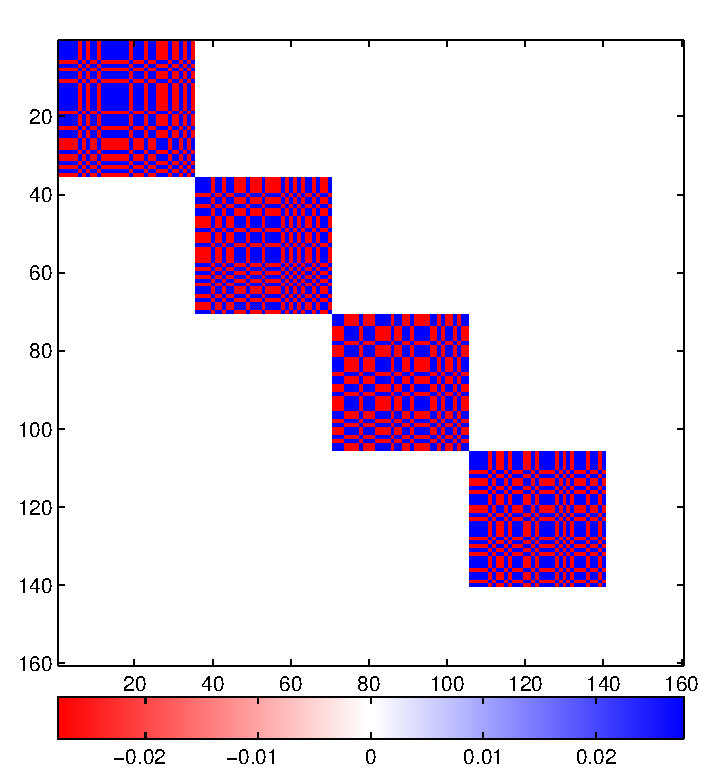
\includegraphics[width=3.5cm]{fig/M} 
  & 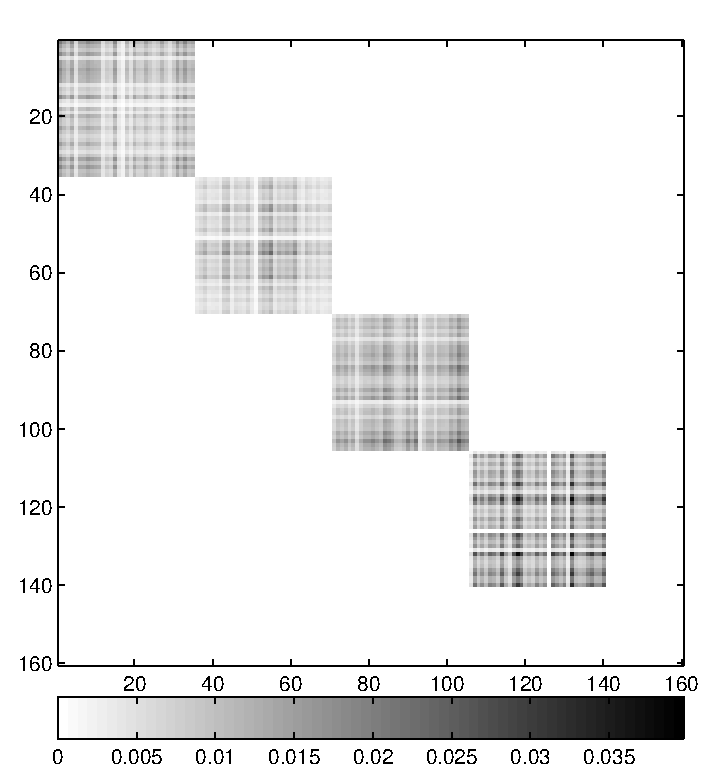
\includegraphics[width=3.5cm]{fig/outputM} 
   \\    (a) & (b) \\[6pt]
\end{tabular}
\caption{\TODO{Experiment on bigger model showing blocks $p = 160$,$n= 2000$,$k = 35$}}
\end{figure}

\subsection{Microarray dataset}

We consider the MILE data \citep{haferlach2010clinical} that measure the mRNA expression levels of 16,853 genes in 541 patients with acute myeloid leukemia (AML), an aggressive blood cancer. The activity of genes is coupled by the activation of biological pathways. This motivates to search for a graphical model with latent variables connected to blocks of genes.

We selected 250 genes with higher variance. We fix the size of the blocks to $k=100$ for our method and compare with the regularized maximum log-likelihood formulation of \citet{chandrasekaran2010}. The obtained empirical covariance matrix has very concentrate eigenvalues and the two first eigenvectors capture most of the covariance. Thus we select parameters for \citet{chandrasekaran2010} such as to recover a low rank component $\hat{L}_{tr}$ of rank two and sparse comonent $\hat{S}_{tr}$  . We then select the parameters of our method such as : to recover a sparse component with comparable level of sparsity as $\hat{S}_{tr}$ (cf. appendix), and a sparse low rank component  $\hat{L}_{ours}$. Figure \ref{fig:gen} shows qualitative results. (a) shows $\hat{L}_{tr}$; (b) shows the low rank sparse component $UU^{\top}$ recovered by our method. For a better visualization of the blocks we have reorered the lines of $U$ such that we group the genes belonging to the same groups. (c) shows $\hat{L}_{ours}$ and (d) shows $\hat{L}_{tr}$ with same order. \citet{chandrasekaran2010} does not recover the block structure while our method provides dense blocks.
%Both methods recover similar block of genes but our method provides more
%and  also genes highly associated with AML: FLT3, NPM1, CEBPA, KIT, N-RAS, MLL, WT1. We fix the size of the blocks to $k=100$ for our method and compare with the regularized maximum log-likelihood. Parameters are chosen so that the two methods recover similar sparse components. Figure \ref{fig:gen} shows qualitative results. (a) shows the low rank sparse component $UU^{\top}$ recovered by our method and (b) is the support of $U$. For a better visualization of the blocks we have reorered the lines of $U$ using Gray code. (c) shows the low rank component estimated by the the regularized maximum log-likelihood and (d) shows this same component reordered according to the blocks found by our method. Both methods seem to recover similar block of genes but our method provides more interpretability.

\begin{figure}
\label{fig:gen}
\center
\begin{tabular}{ccccc}
      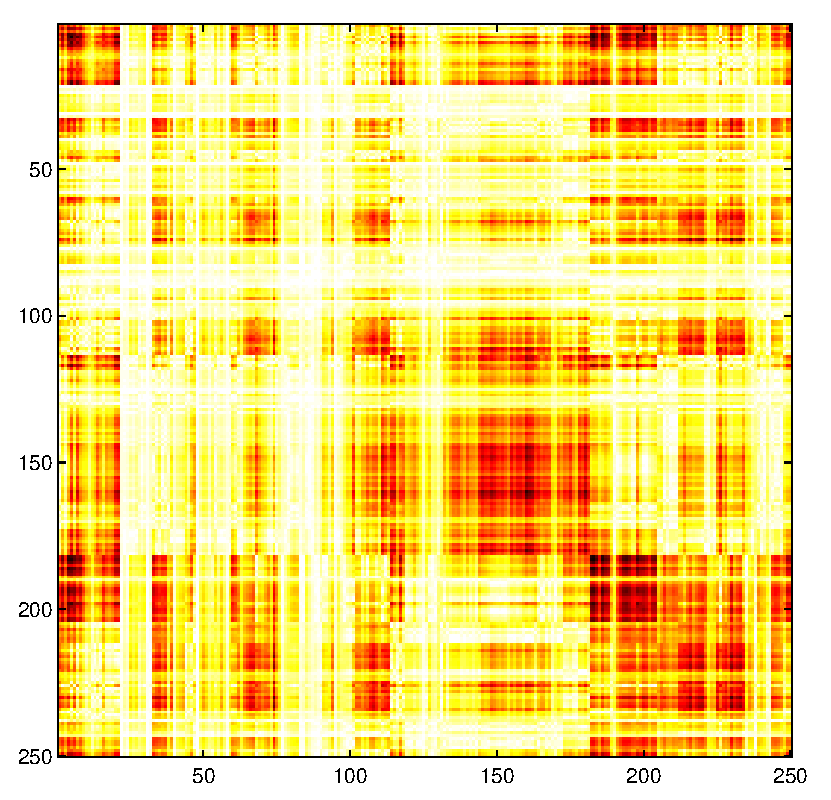
\includegraphics[width=4cm]{fig/MILE_Lsl_not_ordered}
  &   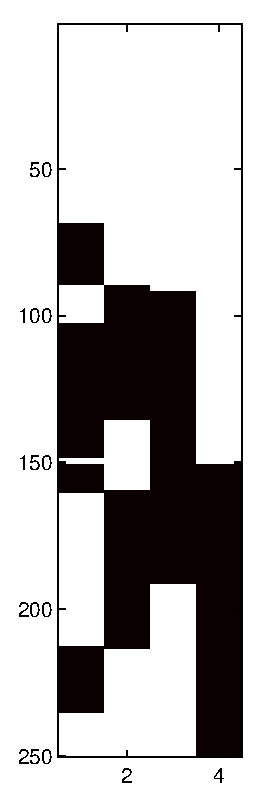
\includegraphics[height=3.8cm]{fig/MILE_blocks}
  &   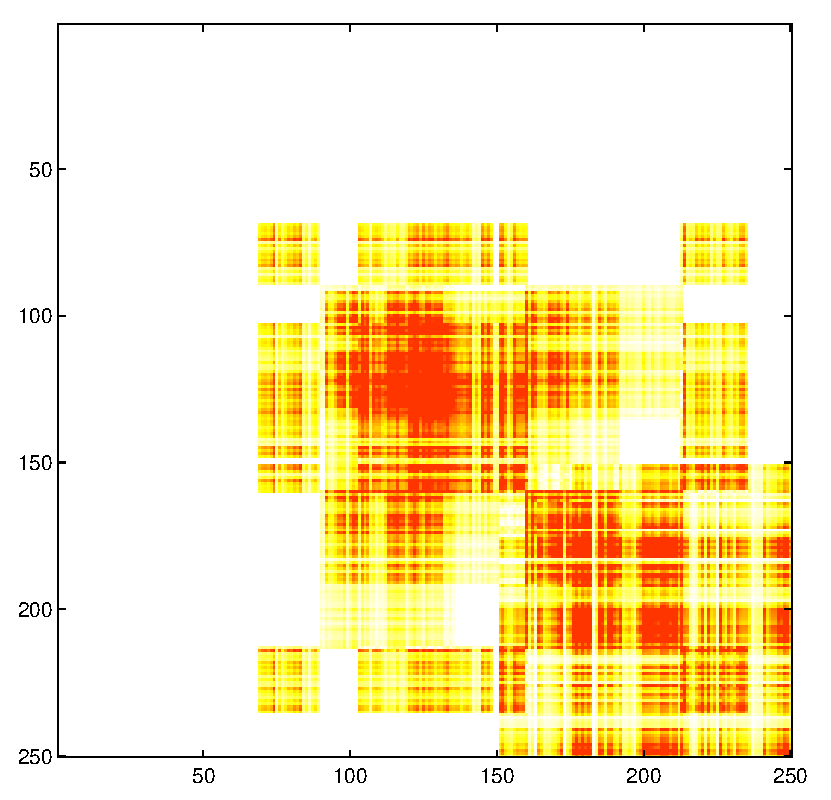
\includegraphics[width=4cm]{fig/MILE_Lom} 
  &   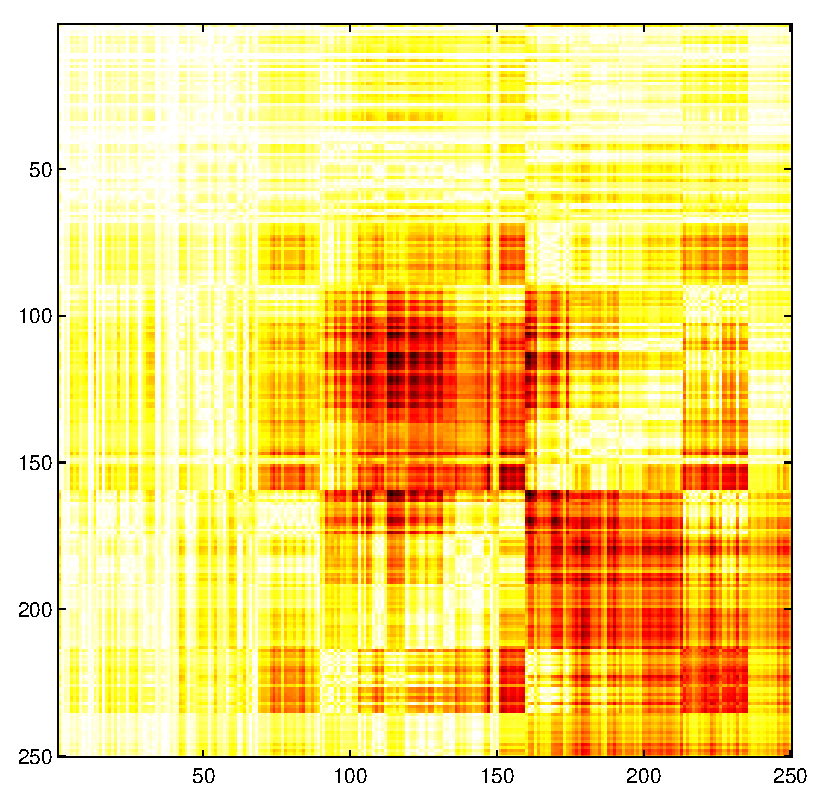
\includegraphics[width=4cm]{fig/MILE_Lsl_ordered} 
  &   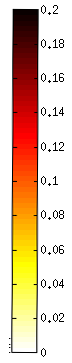
\includegraphics[height=3.8cm]{fig/colorbar} 
   \\   (a)  $\hat{L}_{tr}$  & (b) blocks &(c) $\hat{L}_{ours}$ &(d) $\hat{L}_{tr}$ ordered  
\end{tabular}
\caption{Estimated low rank component $\hat{L}_{tr}$ for \citet{chandrasekaran2010} (a);  the support of the 4 rank-one 100-sparse components $uu^{\top}$ for our estimated low rank component  (b);  our estimated low rank component (d); and $\hat{L}_{tr}$  with the same order as ours }
\end{figure}
